

% --------------------------------------------------------------
\begin{frame}[fragile]
  \frametitle{Motivation}
  \begin{itemize}
    \item LOHS
    \item LOFC
    \item LOHS + LOFC
    \item RIA (or Intentional Reactivity Insertion)
    \item Other transients
  \end{itemize}

\end{frame}

% --------------------------------------------------------------
\begin{frame}[fragile]
  \frametitle{Motivation}
    \begin{itemize}
      \item Characterizing BDBE response is a key requirement for reactor
        licensing.
      \item Key thermal-­‐hydraulic, neutronic, and structural mechanics 
        phenomena differentiate FHRs from other reactor technologies 
      \item The strategy for the FHR methods development program is to use 
        existing codes with extensive design application experience and 
        licensing pedigree 
      \item V\&V of these selected codes must be performed for application to 
        the FHR against experiments with sufficient QA to satisfy the licensing 
        body.  
    \end{itemize}
\end{frame}


% --------------------------------------------------------------
\begin{frame}[fragile]
  \frametitle{Motivation}
  \begin{itemize}
    \item FLiBe coolant
    \item Annular Pebble Fuel with TRISO particles
    \item High Temperatures $>700^{\circ}C$
    \item Strong fuel temperature feedback 
  \end{itemize}

\end{frame}


% --------------------------------------------------------------
\begin{frame}[fragile]
  \frametitle{Motivation}
  \begin{figure}[htbp!]
    \begin{center}
      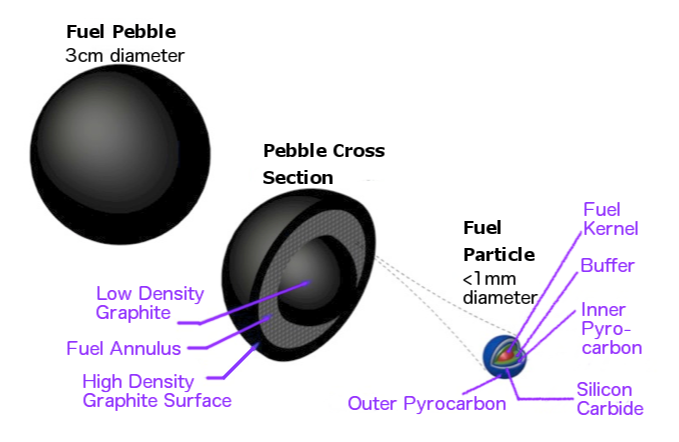
\includegraphics[height=0.7\textheight]{./motivation/fhrpebbles.eps}
    \end{center}
    \caption{Annular Pebble Fuel in the PB-FHR}
    \label{fig:fuel}
  \end{figure}
\end{frame}
